%\documentclass[xcolor={dvipsnames}]{beamer}
\documentclass[9pt]{beamer}
%\usepackage[dvipsnames]{xcolor}
%\usepackage[dvipsnames,table,xcdraw]{xcolor}

\usepackage[utf8]{inputenc}
\usepackage{caption}
\usepackage{tikz}
\usetikzlibrary{tikzmark}
\usetikzlibrary{shapes.geometric}
\usetikzlibrary{arrows,scopes} %tikz libraries used to draw the glyphs
\usetikzlibrary {3d}
\usetikzlibrary{decorations.markings}
\usepackage{circuitikz}
\usepackage{tikz-3dplot}
\usepackage[percent]{overpic}
\usepackage{diagbox}
\usepackage{multirow}
%\usepackage{fontspec}
\usepackage{soul}

\usepackage{hyperref}
\hypersetup{
  colorlinks=true,
  linkcolor=black,
  filecolor=magenta,      
  urlcolor=cyan,
}

\definecolor{green(ryb)}{rgb}{0.4, 0.69, 0.2}

%\usepackage{lmodern}
%\usepackage{helvet}
%\usepackage{gfsneohellenicot}
%\usepackage[light,condensed,math]{kurier}
%\usepackage[T1]{fontenc}
%\usepackage{times}
%\usepackage{tgadventor}
%\usepackage{mathpazo}
%\usepackage{palatino}
\usetheme{Boadilla}
%\usetheme{Montpellier}
%\usetheme{CambridgeUS}
%\usepackage{cmbright}
%\usepackage[OT1]{fontenc}


\usepackage[scaled]{helvet} % With " scaled " option
%\usepackage{eulervm}
%\usefonttheme[onlymath]{serif}
%\usepackage[light,math]{iwona}
%\usepackage[T1]{fontenc}

%\usepackage[sfdefault,lining]{FiraSans} %% option 'sfdefault' activates Fira Sans as the default text font
%\usepackage[fakebold]{firamath-otf}
%\renewcommand*\oldstylenums[1]{{\firaoldstyle #1}}

%\setbeamercolor*{structure}{bg=Green!20,fg=Green}

%\setbeamercolor*{palette primary}{use=structure,fg=white,bg=structure.fg}
%\setbeamercolor*{palette secondary}{use=structure,fg=white,bg=structure.fg!75}
%\setbeamercolor*{palette tertiary}{use=structure,fg=white,bg=structure.fg!50!black}
%\setbeamercolor*{palette quaternary}{fg=white,bg=black}

%\setbeamercolor{section in toc}{fg=black,bg=white}
%\setbeamercolor{alerted text}{use=structure,fg=structure.fg!50!black!80!black}

%\setbeamercolor{titlelike}{parent=palette primary,fg=structure.fg!50!black}
%\setbeamercolor{frametitle}{bg=gray!10!white,fg=PineGreen}

%\setbeamercolor*{titlelike}{parent=palette primary}



%\usetheme{Madrid}
%\usecolortheme{seahorse}
\usecolortheme{dove}
%\usecolortheme{structure}
%\usecolortheme{beetle}
%\usecolortheme{spruce}
%\usecolortheme{fly}
%\usecolortheme{dolphin}
%\usecolortheme{albatross}
%\usefonttheme{serif}

\captionsetup{font=scriptsize,labelfont=scriptsize}


\setbeamertemplate{caption}[numbered]
\setbeamertemplate{itemize item}[circle]
\setbeamertemplate{itemize subitem}[square]
\setbeamertemplate{itemize subsubitem}[triangle]

\newcommand{\backupbegin}{
  \newcounter{finalframe}
  \setcounter{finalframe}{\value{framenumber}}
}
\newcommand{\backupend}{
  \setcounter{framenumber}{\value{finalframe}}
}

%\newcommand{\pt}{$\mathnormal{p}_\mathrm{T}$ }
%\newcommand{\pthat}{$\mathnormal{\hat{p}}_\mathrm{T}$ }
\newcommand{\pt}{$p_{\text{T}}\ $}
\newcommand{\ptjet}{$p_\text{T}^\text{jet}\ $}
\newcommand{\ptmu}{$p_\text{T}^\mu\ $}
\newcommand{\pthat}{$\hat{p}_{\text{T}}\ $}

\newcommand{\rc}{%
  \resizebox{!}{1.25ex}{%
    \begin{tikzpicture}[>=round cap]
      \clip (0.09em,-0.05ex) rectangle (0.61em,0.81ex);
      \draw [line width=.11ex, <->, rounded corners=0.13ex] (0.1em,0.1ex) .. controls (0.24em,0.4ex) .. (0.35em,0.8ex) .. controls (0.29em,0.725ex) .. (0.25em,0.6ex) .. controls (0.7em,0.8ex) and (0.08em,-0.4ex) .. (0.55em,0.25ex);
    \end{tikzpicture}%
  }%
}

\tikzset{middlearrow/.style={
        decoration={markings,
            mark= at position 0.5 with {\arrow{#1}} ,
        },
        postaction={decorate}
    }
}





%Information to be included in the title page:
\title[Thesis Preliminary Exam] %optional
      {\textbf{Thesis Preliminary Exam}}

\author[Clayton Bennett] % (optional, for multiple authors)
       {Clayton Bennett}

\institute[UIC] % (optional)
{
               
  University of Illinois at Chicago \\
  The CMS Collaboration
  
}

\date[4 Dec 2023] % (optional)
     {December 4, 2023}


     \begin{document}
     \graphicspath{ {/home/clayton/Documents/nuclear/GroupMeeting/figures} }

     \begin{frame}
       \titlepage
       \begin{columns}
	 \column{0.2\textwidth}
	 \centering
	 \begin{figure}
	   \includegraphics[width=0.8\textwidth]{CMSlogo}
	 \end{figure}
	 \column{0.6\textwidth}
	 
	 \column{0.2\textwidth}
	 \begin{figure}
	   \includegraphics[width=0.8\textwidth]{UIClogo}
	 \end{figure}
       \end{columns}
     \end{frame}

     \graphicspath{ {/home/clayton/Documents/nuclear/thesisPrelim/figures} }

     \begin{frame}
       \frametitle{\textbf{Outline}}
       %% \begin{itemize}
       %% \item The Quark Gluon Plasma
       %% \item Jets as probes of the Quark Gluon Plasma
       %% \item $b$-jet measurements with CMS
       %% \end{itemize}
       \begin{enumerate}
       \item \label{th1} The Quark Gluon Plasma
       \item \label{th2} Jets as probes of the Quark Gluon Plasma
       \item \label{th3} $b$-jet measurements with CMS
       \end{enumerate}

       \

       \begin{columns}
         \column{0.4\textwidth}
         \begin{tikzpicture}
           \node{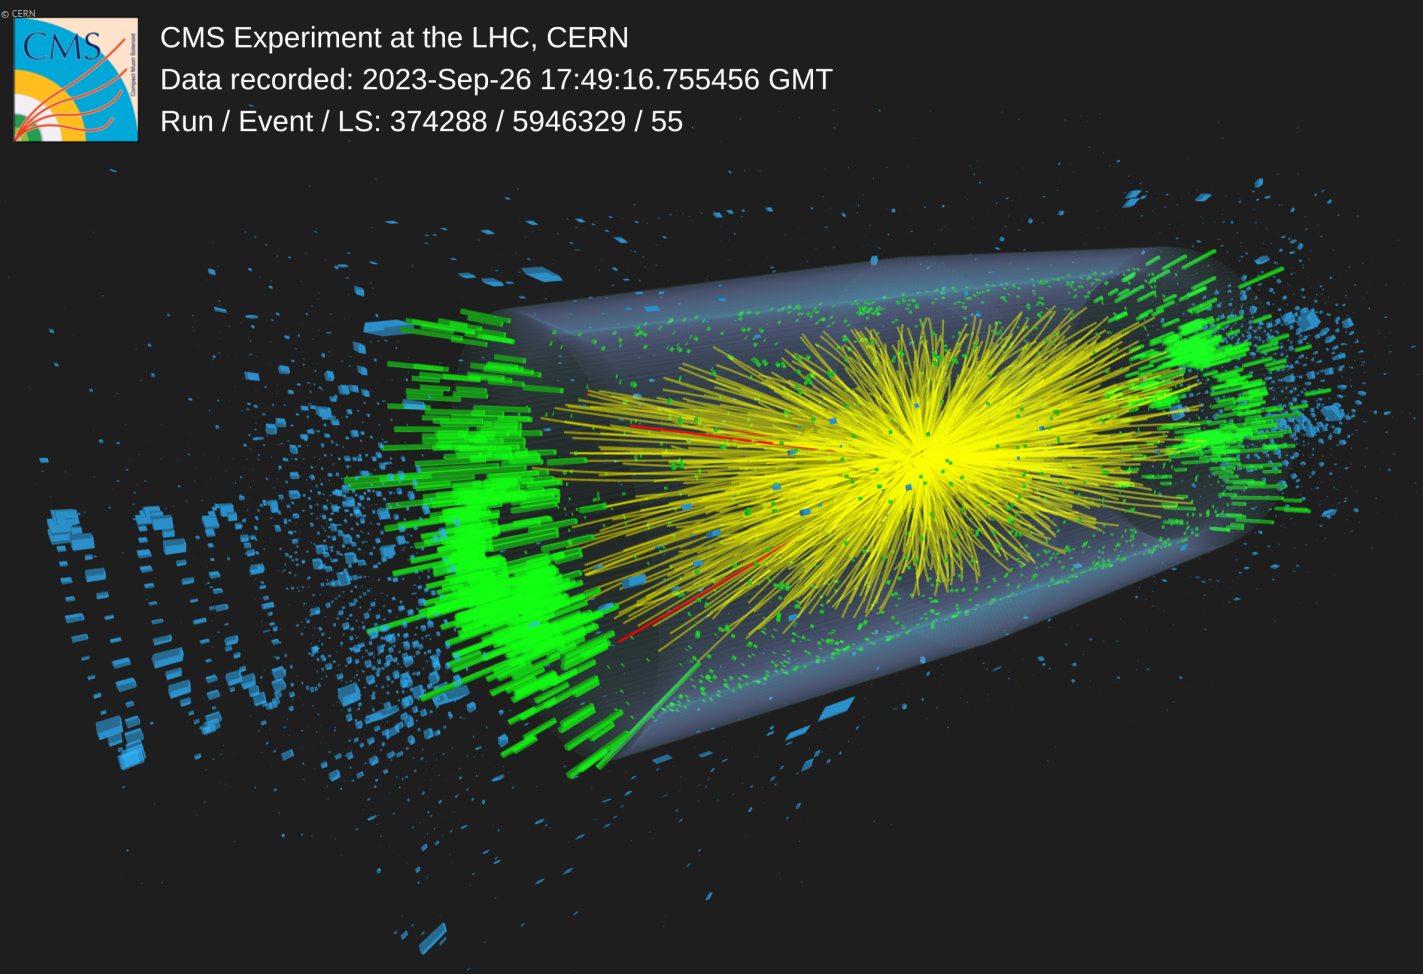
\includegraphics[width=\textwidth]{event-display-1.png}};
         \end{tikzpicture}
         \column{0.4\textwidth}
         \begin{tikzpicture}
           \node{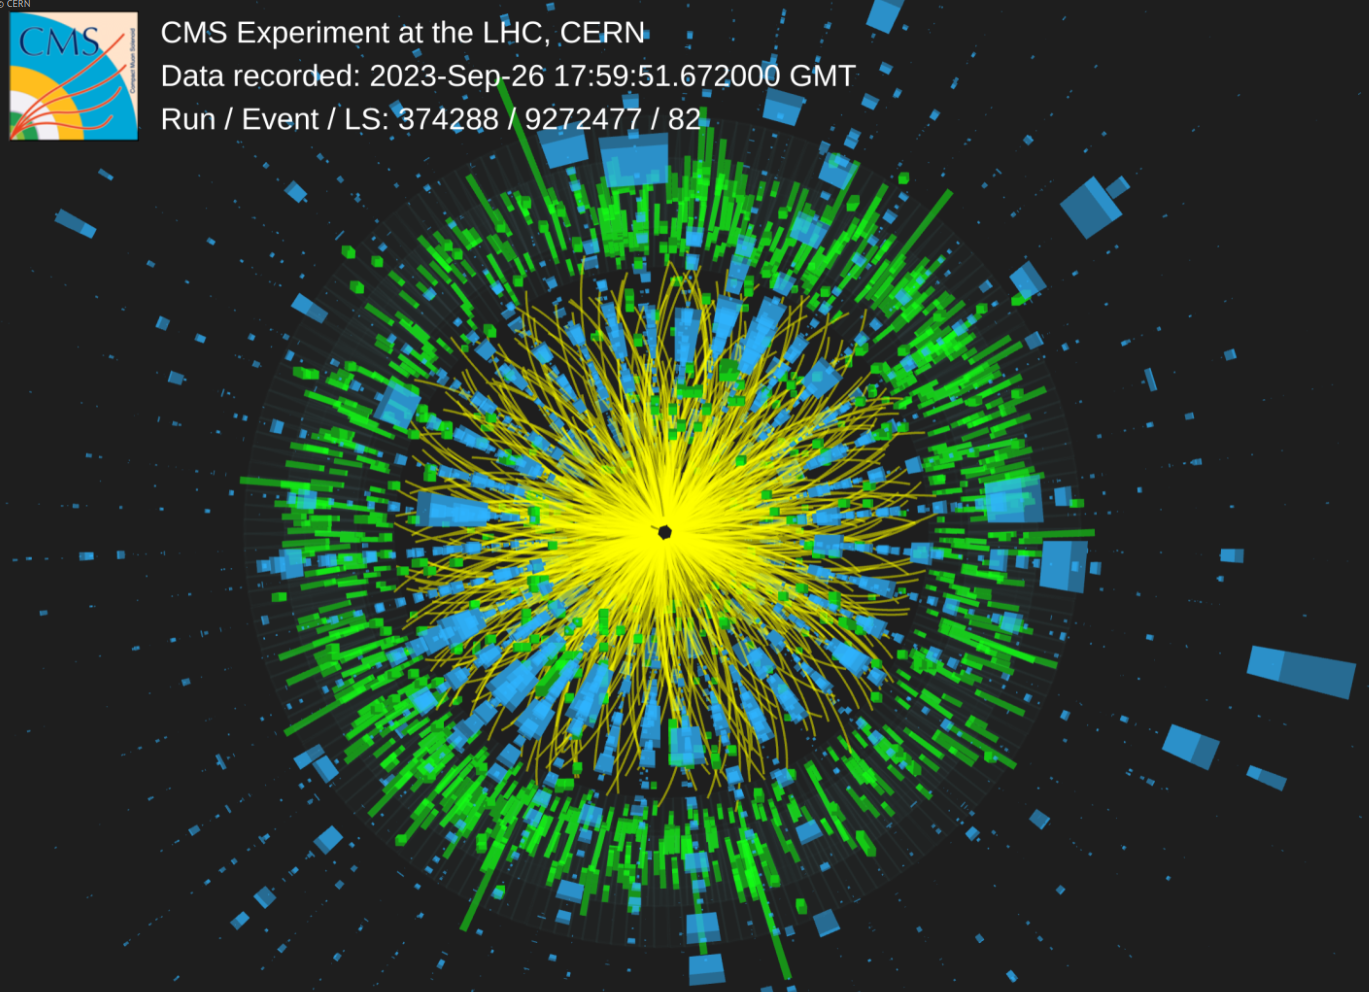
\includegraphics[width=\textwidth]{event-display-2.png}};
         \end{tikzpicture}
       \end{columns}
       \centering \scriptsize First 2023 PbPb collision at 5.36 TeV
     \end{frame}

     \begin{frame}
       \centering \textbf{The Quark Gluon Plasma}
     \end{frame}

     \begin{frame}
       \frametitle{\textbf{The Standard Model of Particle Physics}}
       \begin{columns}
         \column{0.65\textwidth}
         \begin{tikzpicture}
           \node{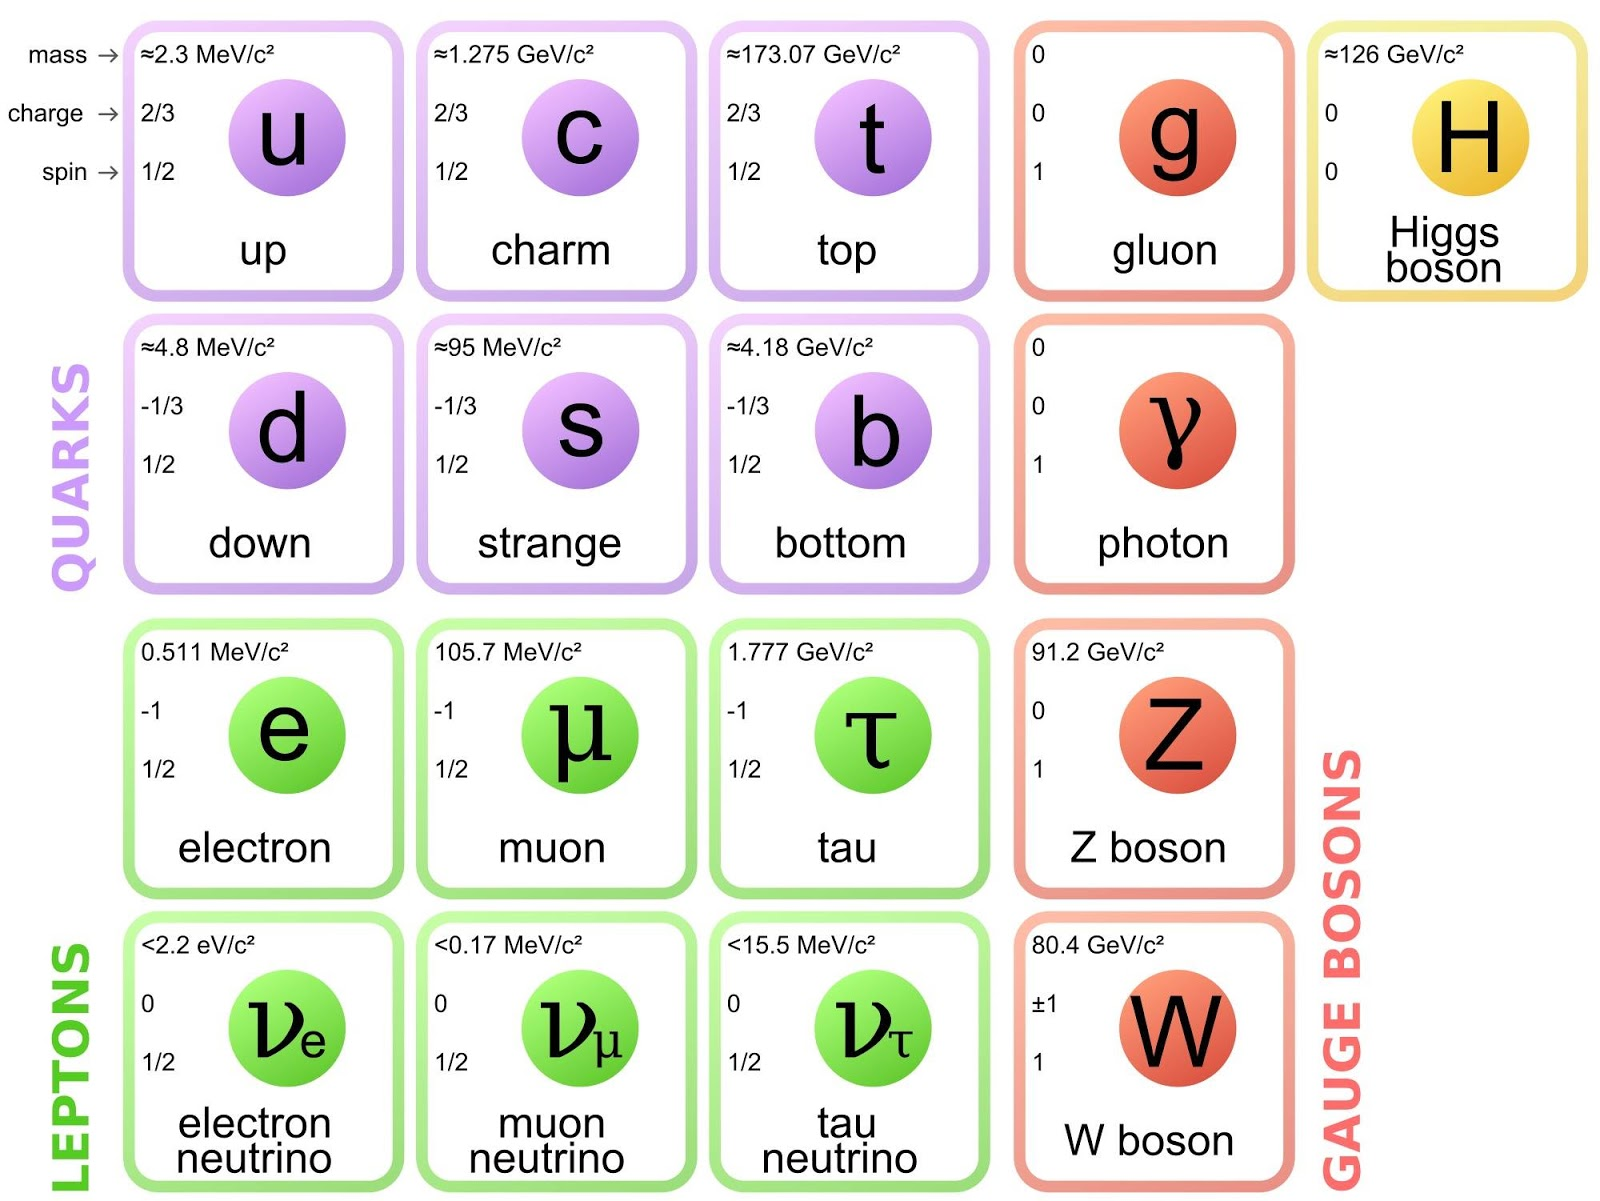
\includegraphics[width=\textwidth]{standard-model.jpg}};
         \end{tikzpicture}
         \column{0.35\textwidth}
         \begin{itemize}
         \item Quantum field theory that describes
           \begin{itemize}
           \item Quantum electrodynamics
           \item Electroweak interactions
           \item Quantum chromodynamics
           \item \st{Gravity}
           \end{itemize}
         \item Quarks and leptons interact via the exchange of gauge bosons
           \begin{itemize}
           \item QED $\to \gamma$
           \item EW $\to W^{\pm}, Z$
           \item QCD $\to g$
           \end{itemize}
         \item $H$ is a mass-giving scalar boson
         \item \textbf{Experimentally verified}
         \end{itemize}
       \end{columns}
     \end{frame}

     \begin{frame}
       \frametitle{\textbf{Quantum Chromodynamics}}
       \begin{columns}
         \column{0.6\textwidth}
         \begin{itemize}
         \item \textbf{Quantum chromodynamics} (QCD) is a quantum field theory describing the \textbf{strong interaction} between \textbf{quarks} and \textbf{gluons}
         \item \textbf{Confinement}: fundamental feature of QCD
           \begin{itemize}
           \item Strong force grows with separationS
           \item $q\bar{q} \to q\bar{q} + q\bar{q}$ (particles from vacuum)
           \end{itemize}
         \item QCD is a quantum field theory with \textbf{asymptotic freedom}
         \end{itemize}
         \begin{align*}
           &\alpha_s(Q^2) = \cfrac{\alpha_s(\mu^2)}{1 + \left[\alpha_s(\mu^2)\frac{(33 - 2n_f)}{12\pi}\right]\ln\left(\frac{Q^2}{\mu^2}\right)} \\
           &\lim_{Q \to \infty}\alpha_s(Q^2) \to 0
         \end{align*}

         \column{0.4\textwidth}
         \centering
         \begin{tikzpicture}
           \node{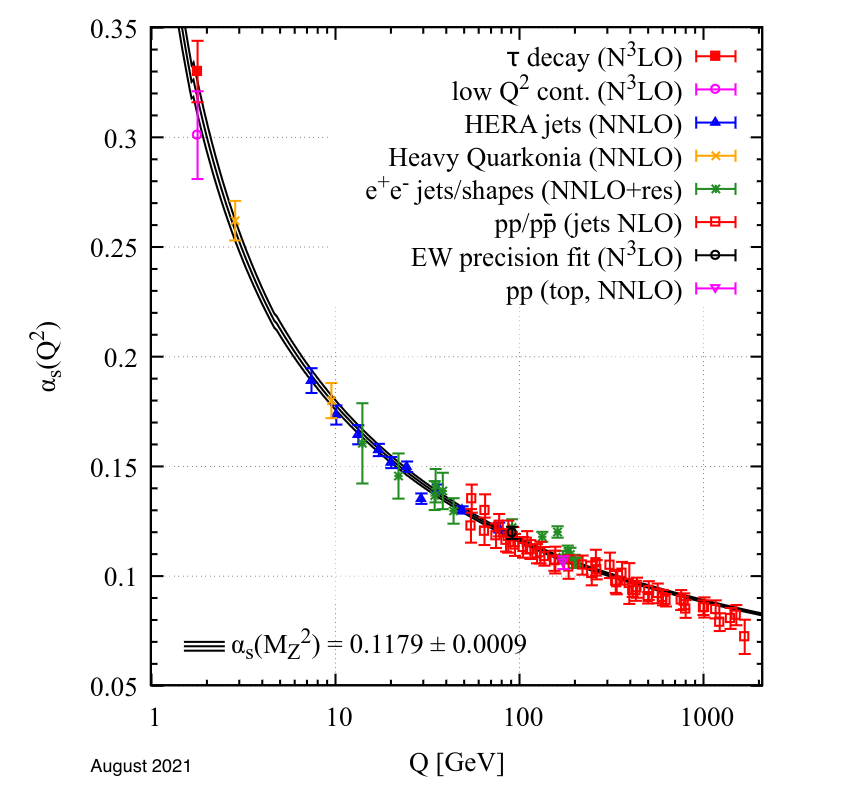
\includegraphics[width=0.9\textwidth]{running-coupling.png}};
           \node[font=\tiny,align=left] at (0.2,2.1) {\href{https://academic.oup.com/ptep/article/2022/8/083C01/6651666}{Prog. Theor. Exp. Phys. 2022, 083C01 (2022)}};
         \end{tikzpicture}

         \

        \begin{tikzpicture}
           \node{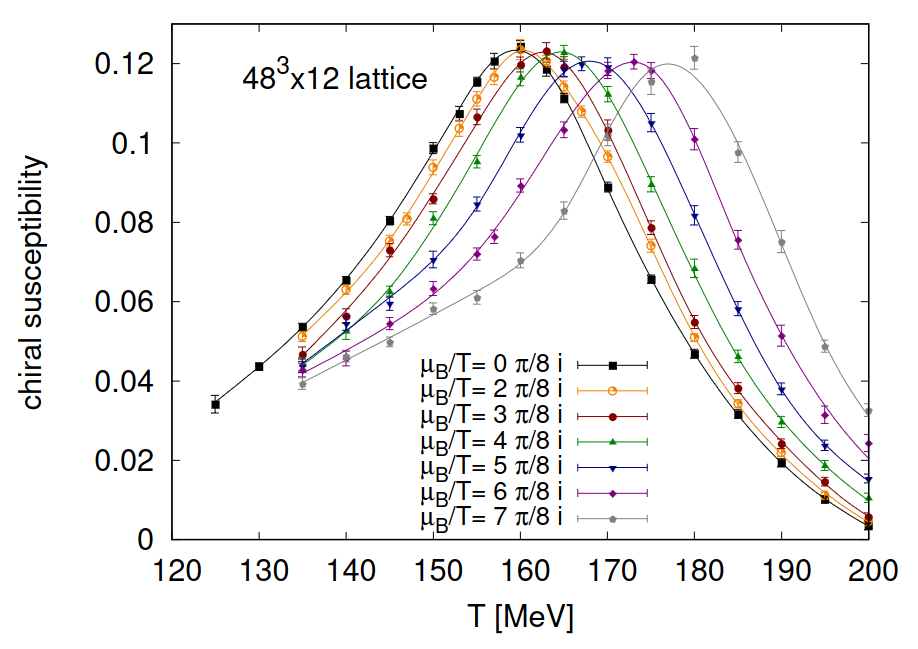
\includegraphics[width=0.9\textwidth]{chiral-susceptibility.png}};
           \node[font=\tiny,align=left] at (1.2,1.6) {\href{https://arxiv.org/abs/2002.02821}{arXiv:2002.02821}};
         \end{tikzpicture}
       \end{columns}
     \end{frame}

     \begin{frame}
       \frametitle{\textbf{Deconfinement}}
       \begin{columns}
         \column{0.5\textwidth}
         \begin{itemize}
         \item 
         \item Lattice QCD predicts a deconfined phase of quarks and gluons known as the \textbf{Quark Gluon Plasma} at extreme temperatures and pressures
         \item At $\mu_B \sim 0$, the critical temperature for this phase-change is $\boldmath{T_c \approx 158.0 \pm 0.6 \textbf{ MeV} \approx 1.8 \cdot 10^{12} \textbf{ K}}$
         \end{itemize}
         \column{0.5\textwidth}
       \end{columns}
     \end{frame}

     \begin{frame}
       \frametitle{\textbf{Phases of QCD}}
       \begin{itemize}
       \item For $\mathbf{\frac{\mu_B}{T} \leq 2}$, QGP-to-hadron phase transition is a \textbf{smooth crossover}
       \item Above some critical point, the QGP-to-hadron transition is expected to become a \textbf{first-order phase transition}
       \end{itemize}

       \

       \centering
       \begin{tikzpicture}
         \node{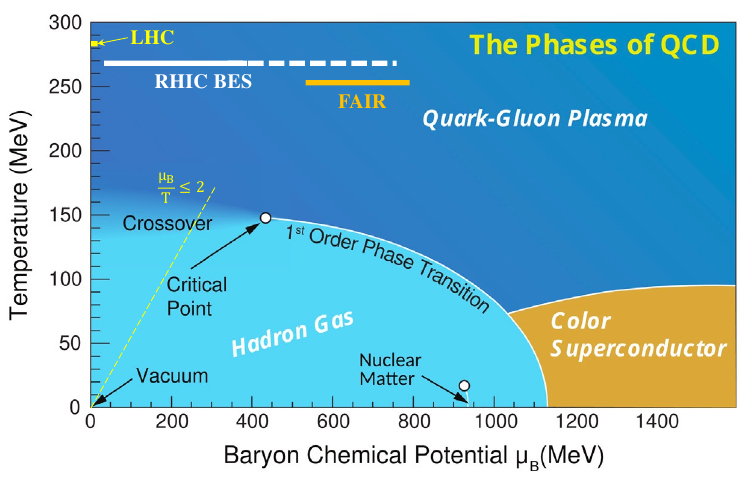
\includegraphics[width=0.8\textwidth]{qcd-phase-diagram.png}};
         \node[font=\tiny,align=left] at (3.5,3) {\href{https://arxiv.org/abs/2303.17254}{arXiv:2303.17254}};
       \end{tikzpicture}
     \end{frame}

     \begin{frame}
       \frametitle{\textbf{QGP at Particle Colliders}}
       \begin{itemize}
       \item We can create QGP in the lab by colliding heavy nuclei ($v \approx c$) in particle accelerators (such as RHIC and LHC)
       \item QCD predicts rich phase dynamics prior to particle detection
         \begin{itemize}
         \item \textbf{Strongly-interacting QGP phase} that flows as a relativistic hydrodynamic fluid
         \item Medium expansion, cooling, and \textbf{hadronization}
         \item Hadronic rescattering and \textbf{freeze-out}
         \end{itemize}
       \end{itemize}

       \
       
       \centering
       \begin{tikzpicture}
         \node{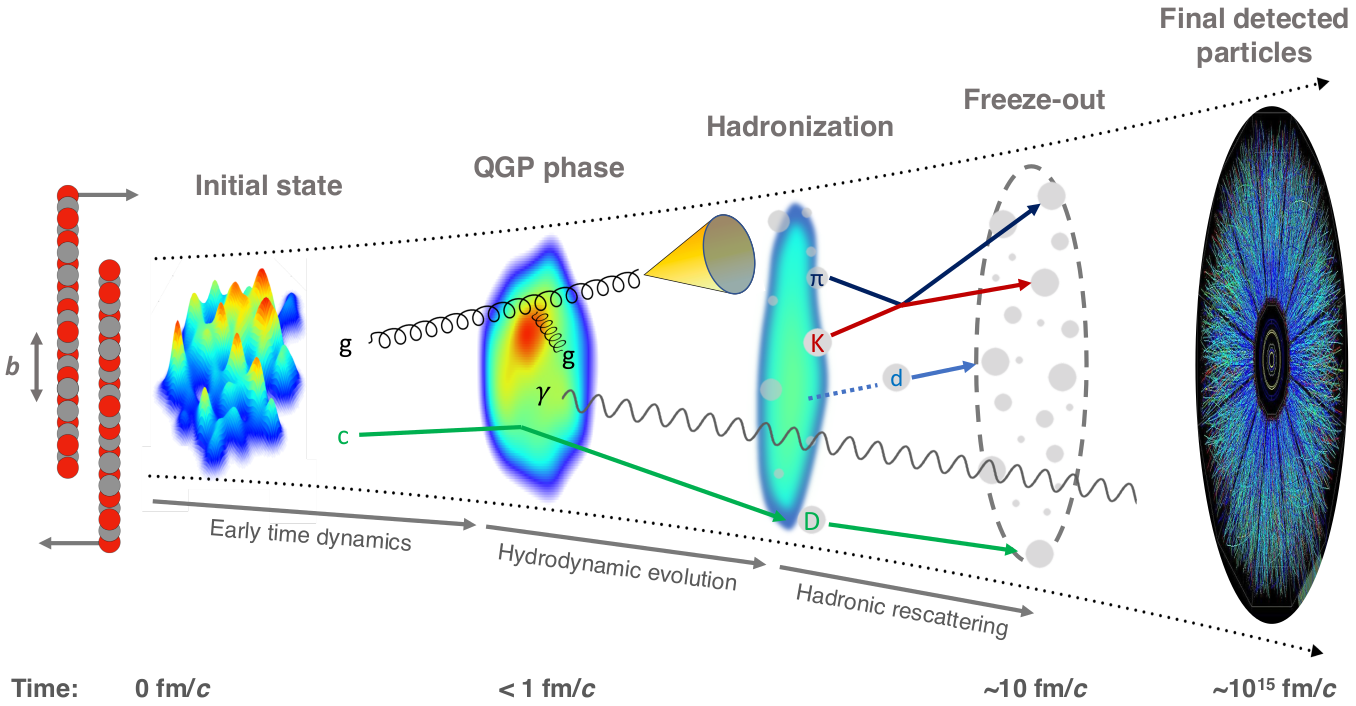
\includegraphics[width=0.8\textwidth]{collision-stages.png}};
       \end{tikzpicture}
     \end{frame}

     \begin{frame}
       \frametitle{\textbf{Kinematics and Centrality}}
       \begin{columns}
         \column{0.4\textwidth}
         \centering
         \newcommand \px {0.6}
         \newcommand \py {1.3}
         \newcommand \pz {0.8}
         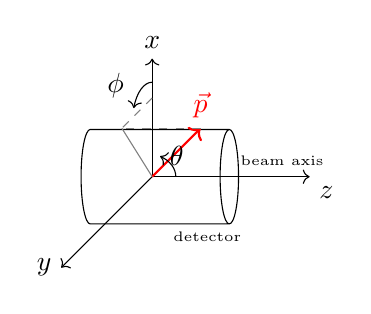
\begin{tikzpicture}
           \tdplotsetmaincoords{70}{110}
           \draw[->] (0,0,0) to (xyz cylindrical cs:radius=2) node[anchor=north west]{$z$};
           \draw[->] (0,0,0) to (xyz cylindrical cs:radius=1.5,angle=90) node[anchor=south]{$x$};
           \draw[->] (0,0,0) to (xyz cylindrical cs:z=3) node[anchor=east]{$y$};
           \node[cylinder, draw, shape aspect=1, minimum height = 2cm, minimum width = 1.2cm] {};
           \draw[->,color=red,thick] (0,0,0) to (\px,\py,\pz) node[color=red,thick,anchor=south]{$\vec{p}$};
           \draw[-,color=gray] (0,0,0) to (0.0,\py,\pz);
           %\draw[-,color=gray] (0,0,0) to (\px,\py,0.0);
           %\draw[-,dashed,color=gray] (\px,\py,\pz) to (\px,\py,0.0);
           \draw[-,dashed,color=gray] (\px,\py,\pz) to (0.0,\py,\pz);
           \draw[-,dashed,color=gray] (0.0,\py,0.0) to (0.0,\py,\pz);
           %\draw[-,dashed,color=gray] (0.0,\py,0.0) to (\px,\py,0.0);
           \draw[->] (.3,0,0) arc [start angle=0,end angle=60,x radius=0.4,y radius=0.3] node[anchor=west]{$\text{  }\theta$};
           \draw[->] (0,1.2,0) arc [start angle=90,end angle=160,x radius=0.25,y radius=0.5] node[anchor=south east]{\ $\phi$};
           \node[font=\tiny] at (0.7,-0.76) {detector};
           \node[font=\tiny] at (1.65,0.2) {beam axis};
         \end{tikzpicture}
         \column{0.6\textwidth}
         \begin{itemize}
         \item Detector geometry warrants the use of cylindrical coordinate system
         \end{itemize}
         \begin{align*}
           \text{transverse momentum} : p_{\text{T}} &= \left|\vec{p}\right| \sin\theta \\
           \text{rapidity} : y &= \cfrac{1}{2} \ln \left( \cfrac{E + p_z}{E - p_z} \right)
           \\
           \text{psuedo-rapidity} :\eta &= \cfrac{1}{2} \ln \left( \cfrac{p + p_z}{p - p_z} \right) \\
           & \to -\ln \left[ \tan\left(\cfrac{\theta}{2}\right) \right]
         \end{align*}
         \begin{itemize}
         \item Why are these variables common in particle physics experiments?
           \begin{itemize}
           \item $\sum_{i} p_{\text{T},i} = 0 + \epsilon$
           \item $y$ is invariant for boosts along $z$-axis
           \end{itemize}
         \end{itemize}
       \end{columns}
       
       
     \end{frame}

     \begin{frame}
       \frametitle{\textbf{Flow in the QGP}}
       \begin{columns}
         \column{0.5\textwidth}
         \begin{itemize}
         \item QGP is a hydrodynamic fluid $\to$ initial spacial anisotropies result in momentum-space anisotropies
         \item $v_n$ measurements quantify the $\phi$-space anisotropy
         \end{itemize}
         \begin{align*}
           \cfrac{dN}{d\phi} = A \cdot \left( 1 + 2\sum_{n = 1}^{\infty} v_n \cos\left[n(\phi - \bar{\Psi}_{n})\right]   \right) 
         \end{align*}
         \begin{itemize}
           \item Flow harmonics $v_n$ are observed to scale with parton number $\to$ further evidence of deconfinement
         \end{itemize}
         \column{0.5\textwidth}
         \begin{tikzpicture}
           \node{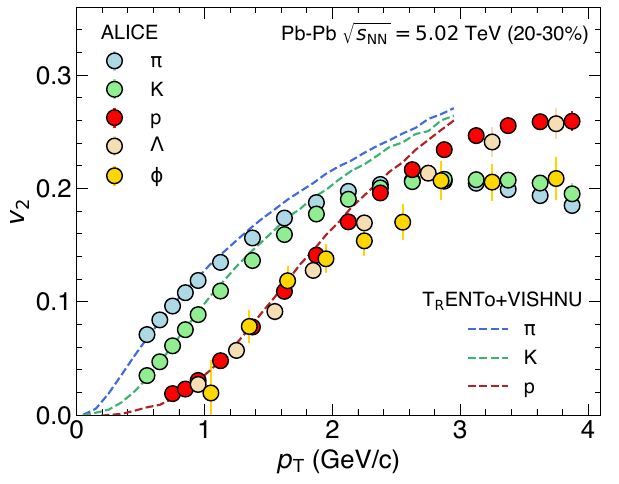
\includegraphics[width=\textwidth]{v2.png}};
         \end{tikzpicture}
       \end{columns}
     \end{frame}

     \begin{frame}
       \centering \textbf{Jets as Probes of the QGP}       
     \end{frame}

     \begin{frame}
       \frametitle{\textbf{Factorization Theorems in QCD}}
       
       \begin{itemize}
       \item \textbf{Hard processes in pp} $\to$ \color{blue} short-distance physics \color{black} of partons $\bigotimes$ \color{red} long-distance phyiscs \color{black} of hadrons
       \end{itemize}

       \
       
       \centering Cross-section factorization in pp collisions
       \begin{align*}
         d\sigma^{p+p \to h + X} &= \sum_f \color{blue}d\sigma^{p+p \to f + X} \color{black}\bigotimes \color{red}D_{f \to h} (z, \mu_F^2) \\
        \color{black} &= \sum_{\color{blue}i,j,k\color{black},f,...}\color{blue} f_{i/p}(x_1,Q^2) \bigotimes f_{j/p}(x_2,Q^2) \bigotimes \hat{\sigma}_{ij\to f + k ...} \color{black}\bigotimes \color{red}D_{f \to h} (z, \mu_F^2)
       \end{align*}
       \begin{itemize}
       \item We use hard processes in pp collisions as a reference when we study QGP medium effects
       \end{itemize}
       \begin{columns}
         \column{0.6\textwidth}
         \centering
         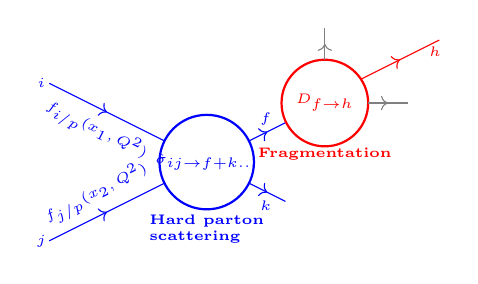
\begin{tikzpicture}
           \draw[-,blue,middlearrow={>}] (-2,1) to (-0.5366,0.2683);
           \draw[-,blue,middlearrow={>}] (-2,-1) to (-0.5366,-0.2683);
           \draw[blue,thick] (0,0) circle (0.6) node[font=\tiny]{$\hat{\sigma}_{ij\to f + k ...}$};
           \draw[-,blue,middlearrow={>}] (0.5366,0.2683) to (1,0.5);
           \draw[-,blue,middlearrow={>}] (0.5366,-0.2683) to (1,-0.5);
           %\draw[rotate=120,blue] (0,0) circle(0.5cm and 0.2cm);
           \draw[red,thick] (1.5,0.75) circle (0.55) node[font=\tiny]{$D_{f \to h}$};
           \draw[-,red,middlearrow={>}] (1.953,1.05) to (2.953,1.55);
           \draw[-,gray,middlearrow={>}] (1.5,1.3) to (1.5,1.7);
           \draw[-,gray,middlearrow={>}] (2.05,0.75) to (2.55,0.75);
           \node[font=\tiny,blue,align=left] at (0,-0.85) {\textbf{Hard parton} \\ \textbf{scattering}};
           \node[font=\tiny,red,align=left] at (1.5,0.1) {\textbf{Fragmentation}};
           \node[font=\tiny,blue,rotate=-26.56] at (-1.4,0.4) {$f_{i/p}(x_1,Q^2)$};
           \node[font=\tiny,blue,rotate=26.56] at (-1.4,-0.4) {$f_{j/p}(x_2,Q^2)$};
           \node[font=\tiny,red] at (2.9,1.4) {$h$};
           \node[font=\tiny,blue] at (-2.1,1) {$i$};
           \node[font=\tiny,blue] at (-2.1,-1) {$j$};
           \node[font=\tiny,blue] at (0.75,-0.55) {$k$};
           \node[font=\tiny,blue] at (0.75,0.55) {$f$};
         \end{tikzpicture}
         \column{0.4\textwidth}
         \begin{itemize}
         \item Cross-section in vacuum is perturbatively calculable!
         \item Fragmentation is non-perturbative $\to$ must rely on QCD-inspired models
         \end{itemize}
       \end{columns}
       
     \end{frame}

     \begin{frame}
       \frametitle{\textbf{Factorization Theorems in QCD}}

       \begin{itemize}
       \item \textbf{Hard processes in AA} $\to$ \color{blue} short-distance physics \color{black} of partons $\bigotimes$ \color{magenta} Model-dependent energey loss \color{black} of partons in the QGP $\bigotimes$ \color{red} long-distance phyiscs \color{black} of hadrons
       \end{itemize}

       \
       
       \centering Cross-section factorization in AA collisions
       \begin{align*}
         d\sigma^{A+A \to h + X} &= \sum_f \color{blue}d\sigma^{A+A \to f + X}_{(\text{vac})} \color{black}\bigotimes \color{magenta} P_f(\Delta E, L, \hat{q}) \color{black} \bigotimes \color{red}D_{f \to h}^{(\text{vac})} (z, \mu_F^2) 
       \end{align*}
       \begin{columns}
         \column{0.6\textwidth}
         \centering
         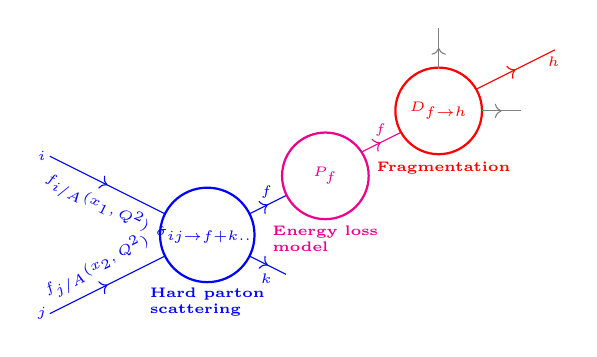
\begin{tikzpicture}
           \draw[-,blue,middlearrow={>}] (-2,1) to (-0.5366,0.2683);
           \draw[-,blue,middlearrow={>}] (-2,-1) to (-0.5366,-0.2683);
           \draw[blue,thick] (0,0) circle (0.6) node[font=\tiny]{$\hat{\sigma}_{ij\to f + k ...}$};
           \draw[-,blue,middlearrow={>}] (0.5366,0.2683) to (1,0.5);
           \draw[-,blue,middlearrow={>}] (0.5366,-0.2683) to (1,-0.5);
           %\draw[rotate=120,blue] (0,0) circle(0.5cm and 0.2cm);
           \draw[magenta,thick] (1.5,0.75) circle (0.55) node[font=\tiny]{$P_f$};
           \draw[-,magenta,middlearrow={>}] (1.953,1.05) to (2.453,1.3);
           \node[font=\tiny,magenta] at (2.2,1.33) {$f$};
           \node[font=\tiny,blue,align=left] at (0,-0.85) {\textbf{Hard parton} \\ \textbf{scattering}};
           \node[font=\tiny,magenta,align=left] at (1.5,-0.05) {\textbf{Energy loss} \\ \textbf{model}};
           \node[font=\tiny,blue,rotate=-26.56] at (-1.4,0.4) {$f_{i/A}(x_1,Q^2)$};
           \node[font=\tiny,blue,rotate=26.56] at (-1.4,-0.4) {$f_{j/A}(x_2,Q^2)$};
           \node[font=\tiny,blue] at (-2.1,1) {$i$};
           \node[font=\tiny,blue] at (-2.1,-1) {$j$};
           \node[font=\tiny,blue] at (0.75,-0.55) {$k$};
           \node[font=\tiny,blue] at (0.75,0.55) {$f$};
           \draw[red,thick] (2.939,1.575) circle (0.55) node[font=\tiny]{$D_{f \to h}$};
           \draw[-,red,middlearrow={>}] (3.415,1.85) to (4.415,2.35);
           \node[font=\tiny,red] at (4.4,2.2) {$h$};
           \draw[-,gray,middlearrow={>}] (2.939,2.125) to (2.939,2.625);
           \draw[-,gray,middlearrow={>}] (3.489,1.575) to (3.989,1.575);
           \node[font=\tiny,red,align=left] at (3,0.85) {\textbf{Fragmentation}};
         \end{tikzpicture}
         \column{0.4\textwidth}
         \begin{itemize}
         \item Factorization theorems unkown for processes embedded in a QGP medium
         \item Energy loss mechanisms
           \begin{itemize}
           \item Collisional energy loss
             \begin{itemize}
             \item Elastic scattering with medium
             \item Dominant for heavy quarks
             \end{itemize}
           \item Radiative energy loss
             \begin{itemize}
             \item Inelastic scattering with medium (gluon Bremsstrahlung)
             \item Dominant for light quarks
             \end{itemize}
           \end{itemize}
         \end{itemize}
       \end{columns}
     \end{frame}

     \begin{frame}
       \frametitle{\textbf{Jets}}
     \end{frame}

     \begin{frame}
       \frametitle{\textbf{Charged Particle Suppression}}
       \begin{columns}
         \column{0.5\textwidth}
         \begin{itemize}
         \item Charged partons lose energy as they traverse the QGP via color interactions
         \item This results in reduced charged-particle yields in AA collisions as compared to pp
           \begin{itemize}
           \item Strong $p_{\text{T}}$ dependence
           \end{itemize}
         \item Colorless probes can be used as reference
         \end{itemize}
         \begin{align*}
           R_{\text{AA}}^{\text{ch}} (p_{\text{T}}) = \cfrac{dN^{\text{AA}}_{\text{ch}} / dp_{\text{T}}}{\left< N_{\text{coll}} \right> dN^{\text{pp}}_{\text{ch}} / dp_{\text{T}}}
         \end{align*}
         \column{0.5\textwidth}
         \begin{tikzpicture}
           \node{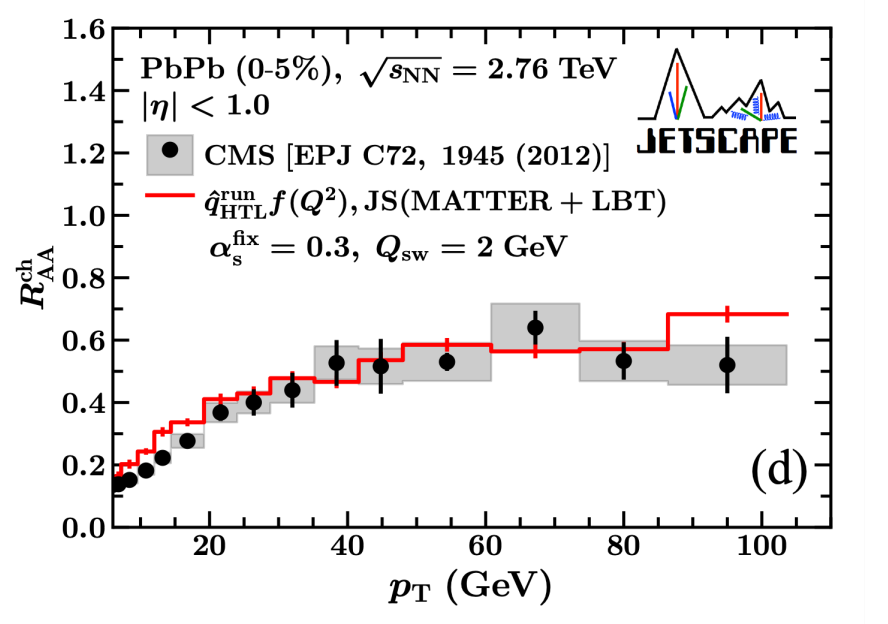
\includegraphics[width=\textwidth]{charged-hadron-RAA.png}};
         \end{tikzpicture}
       \end{columns}
     \end{frame}

     \begin{frame}
       \frametitle{\textbf{Jet suppression}}
       \begin{columns}
         \column{0.5\textwidth}
         \begin{itemize}
         \item Leading hadron measurements do not fully connect to the initial fragmenting parton
         \item Suppression of fully reconstructed jets is a better probe
           \begin{itemize}
           \item Weak $p_{\text{T}}$ dependence
           \item Scales with centrality
           \end{itemize}
         \end{itemize}
         \begin{align*}
           R_{\text{AA}}^{\text{jet}} (p_{\text{T}}) = \cfrac{dN^{\text{AA}}_{\text{jet}} / dp_{\text{T}}}{\left< N_{\text{coll}} \right> dN^{\text{pp}}_{\text{jet}} / dp_{\text{T}}}
         \end{align*}
         \column{0.5\textwidth}
         \begin{tikzpicture}
           \node{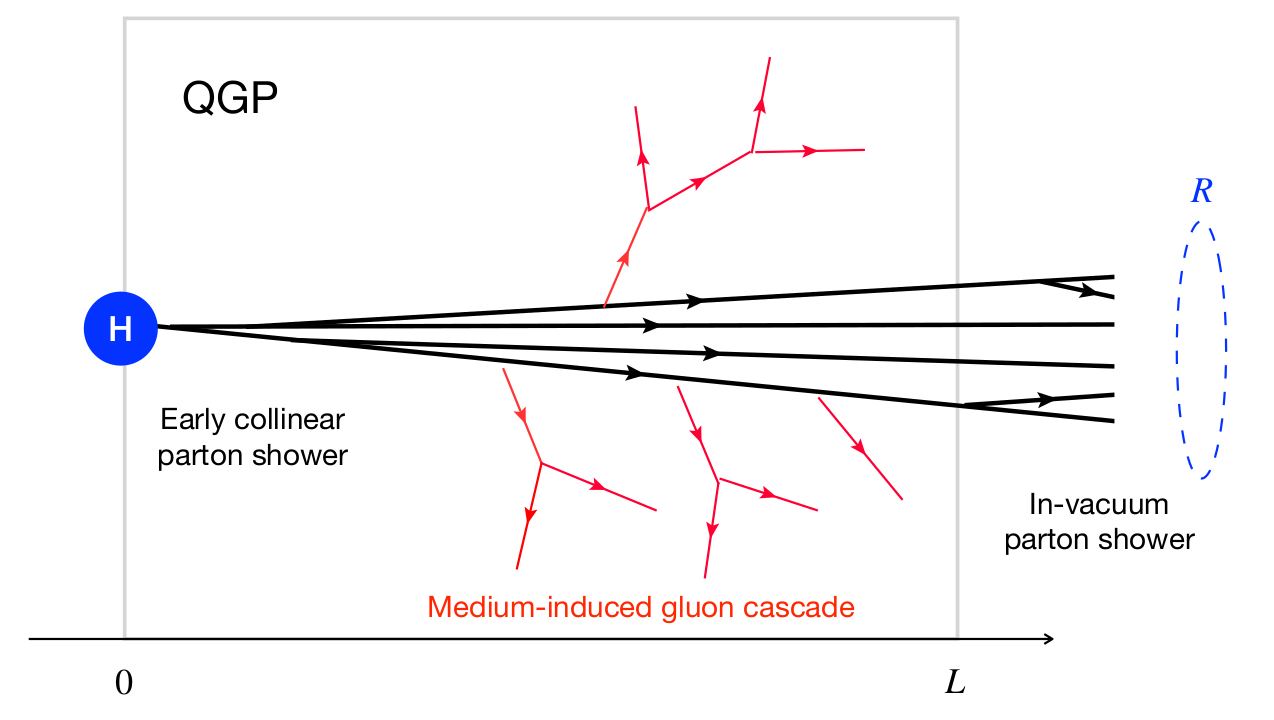
\includegraphics[width=\textwidth]{jet-suppression-cartoon.png}};
         \end{tikzpicture}
       \end{columns}
       \begin{columns}
         \column{0.5\textwidth}
         \begin{tikzpicture}
           \node{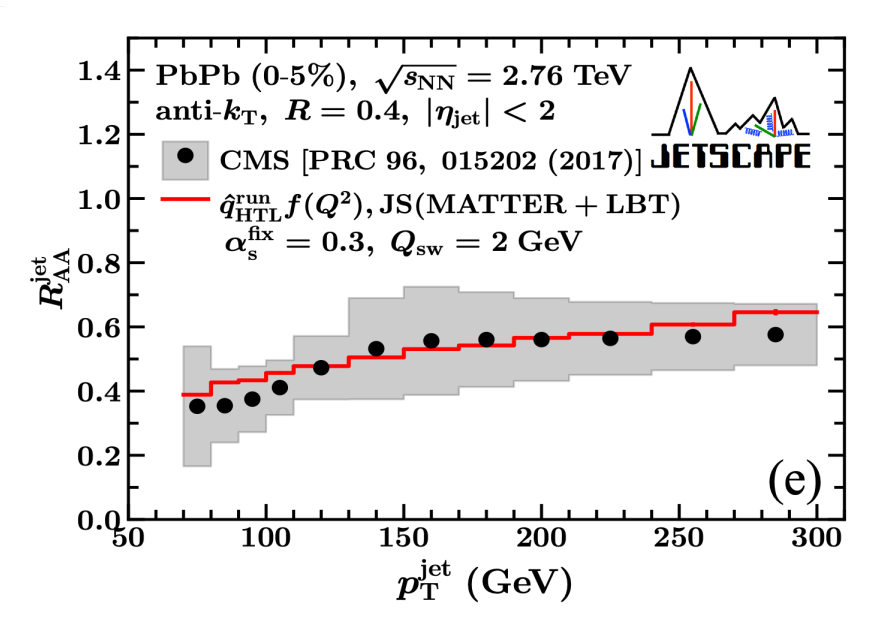
\includegraphics[width=\textwidth]{jet-RAA.png}};
         \end{tikzpicture}
         \column{0.5\textwidth}
         \begin{tikzpicture}
           \node{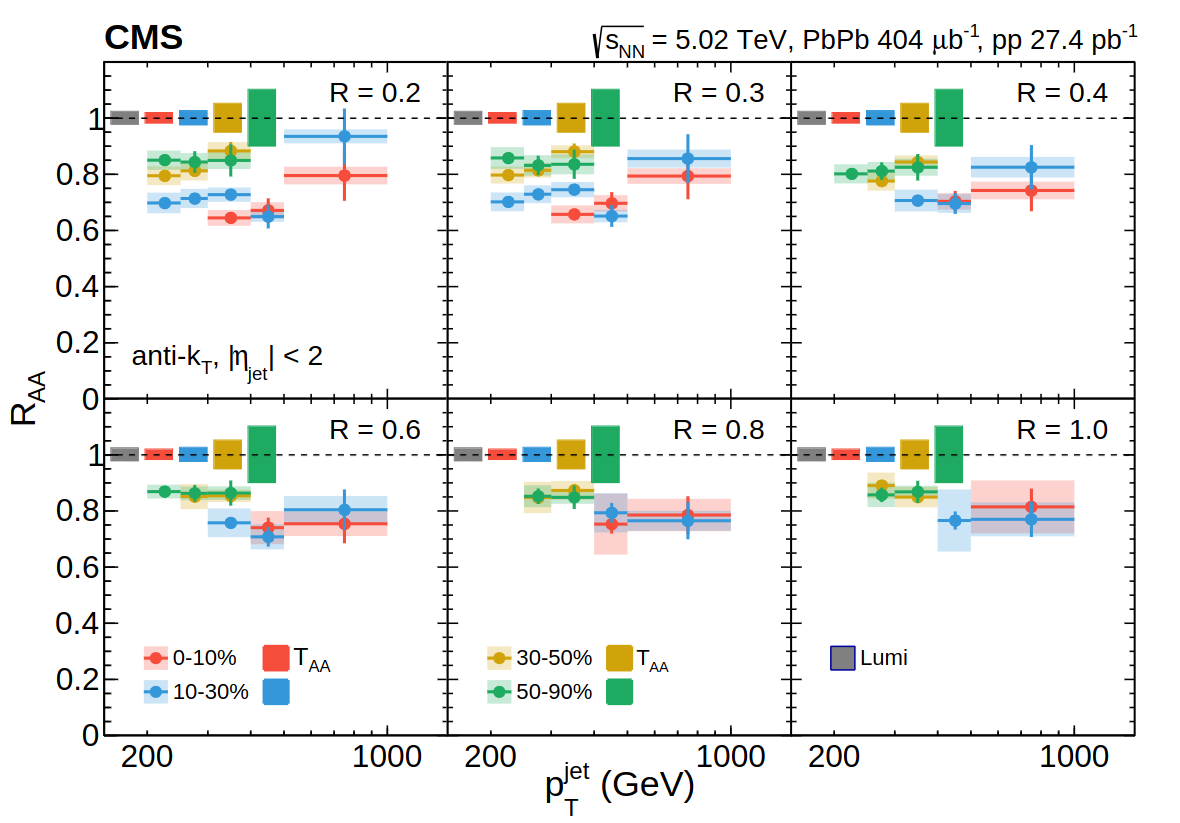
\includegraphics[width=\textwidth]{jet-radii-RAA.png}};
         \end{tikzpicture}
       \end{columns}
     \end{frame}

     \begin{frame}
       \frametitle{\textbf{$b$-jet Indetification}}
     \end{frame}

     \begin{frame}
       \frametitle{\textbf{Muon rel-$p_{\text{T}}$}}
     \end{frame}

     \begin{frame}
       \centering \textbf{$b$-jet measurements with CMS}
       \begin{itemize}
       \item Jets resulting from a framgenting $b$-quark are interesting objects because they are good tests many theories
         \begin{itemize}
         \item Heavy flavor QCD
         \item B-meson physics
         \end{itemize}
       \item Many methods have been deployed to identify $b$-jets
         \begin{itemize}
         \item Impact Parameter (IP) Significance
           \begin{itemize}
           \item IP is the distance between the primary vertex and the point of closest approach of a track
           \item $b$-jets tend to have wider IP distributions
           \end{itemize}
         \item Secondary Vertex Reconstruction
           \item $b$-jets tend to have secondary vertices due to in-flight decays
         \item Jet Probability
         \item Soft Lepton Tagging
         \item Deep Learning Techniques
         \end{itemize}
       \end{itemize}
     \end{frame}

     \begin{frame}
       \frametitle{\textbf{CMS Detector}}
       \centering \begin{tikzpicture}
         \node{\includegraphics[width=0.9\textwidth]{cms-detector.png}};
         \node[font=\tiny] at (4,3.5) {\href{https://arxiv.org/abs/1706.04965}{arXiv:1706.04965}};
       \end{tikzpicture}
     \end{frame}
     
     \begin{frame}
       \frametitle{\textbf{CMS Detector}}
       \centering \begin{tikzpicture}
         \node{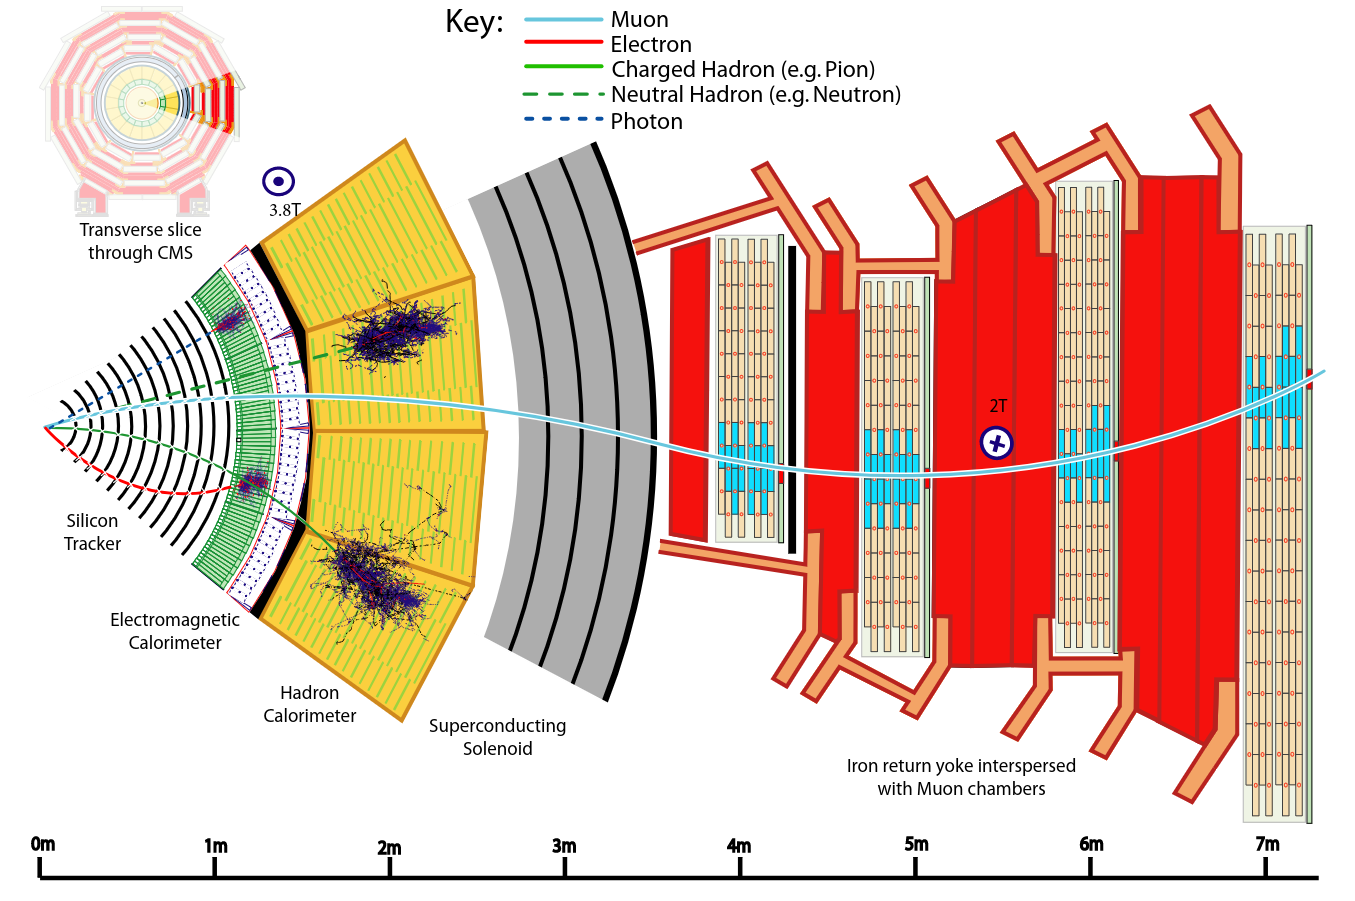
\includegraphics[width=0.9\textwidth]{cms-detector-slice.png}};
         \node[font=\tiny] at (4,3.5) {\href{https://arxiv.org/abs/1706.04965}{arXiv:1706.04965}};
       \end{tikzpicture}
     \end{frame}

     \begin{frame}
       \frametitle{\textbf{Jet Reconstruction in Heavy Ion Collisions}}
     \end{frame}

     \end{document}
